\chapter{Pattern Recognition}

% **************************** Define Graphics Path **************************

\epstopdfsetup{outdir=Chapter3/Figs/PDF/}
\ifpdf
    \graphicspath{{Chapter3/Figs/Raster/}{Chapter3/Figs/PDF/}{Chapter3/Figs/}}
\else
    \graphicspath{{Chapter3/Figs/Vector/}{Chapter3/Figs/}}
\fi

\section{Improved Contour Detection}\label{sec:ImprovedContourDetection}

OpenCV's findContours method takes a binary image and finds the contours in that binary image. However, the problem with this method is that we're thresholding on chromatic values, i.e. using color information to break up the color information into blobs off of which we're finding the contours. This doesn't take into account the white-out and black-out, which was noted previously. It's straightforward to define regions in the image which are succeptible to white-out and black-out using the luminosity channel. This is done by taking a high and low threshold off the luminosity channel, thereby producing a binary image, which is 1 in the valid region, and 0 otherwise.

We take that, and we add it to our thresholded chromatic channel, which produces a 2-bit image. For this purpose, a 2-bit data type was added to OpenCV. The question then is how to use it. Essentially, we have four different states: values which are neither the right color nor in the right region; values which are possibly the right color, but because they're outside the valid region, they've potentially suffered from white-out and black-out and as such they are not reliable indicators for either the start of an edge or the end of an edge; values which are in the right region, but the wrong color, and we are certain that they are not skin; and finally, values which are in the valid region and are of the right color.

The Canny edge detector method is perfect for implementing a decision by setting a high threshold --- our strong criteria --- in the right region in the right color, and a low threshold so that it will continue following an edge across values which are in the invalid region. Whichever value we set the low threshold to depends on the state of the image; we use a lower value if there is ambiguity and a higher value if the result is fairly accurate:

\begin{center}
\begin{tabular}{|c|c|c|c||c|c|}
\hline
\multicolumn{2}{|c|}{Image} & Color & Region & \multicolumn{2}{|c|}{Bit}\\\hline
0 & 0 & 0 & 1 & Color & XAND(Color, Region)\\\hline
0 & 1 & 0 & 0 & Color & XAND(Color, Region)\\\hline
1 & 0 & 1 & 0 & Color & XAND(Color, Region)\\\hline
1 & 1 & 1 & 1 & Color & XAND(Color, Region)\\\hline
\end{tabular}
\end{center}

\begin{figure}[h!]
  \centering
    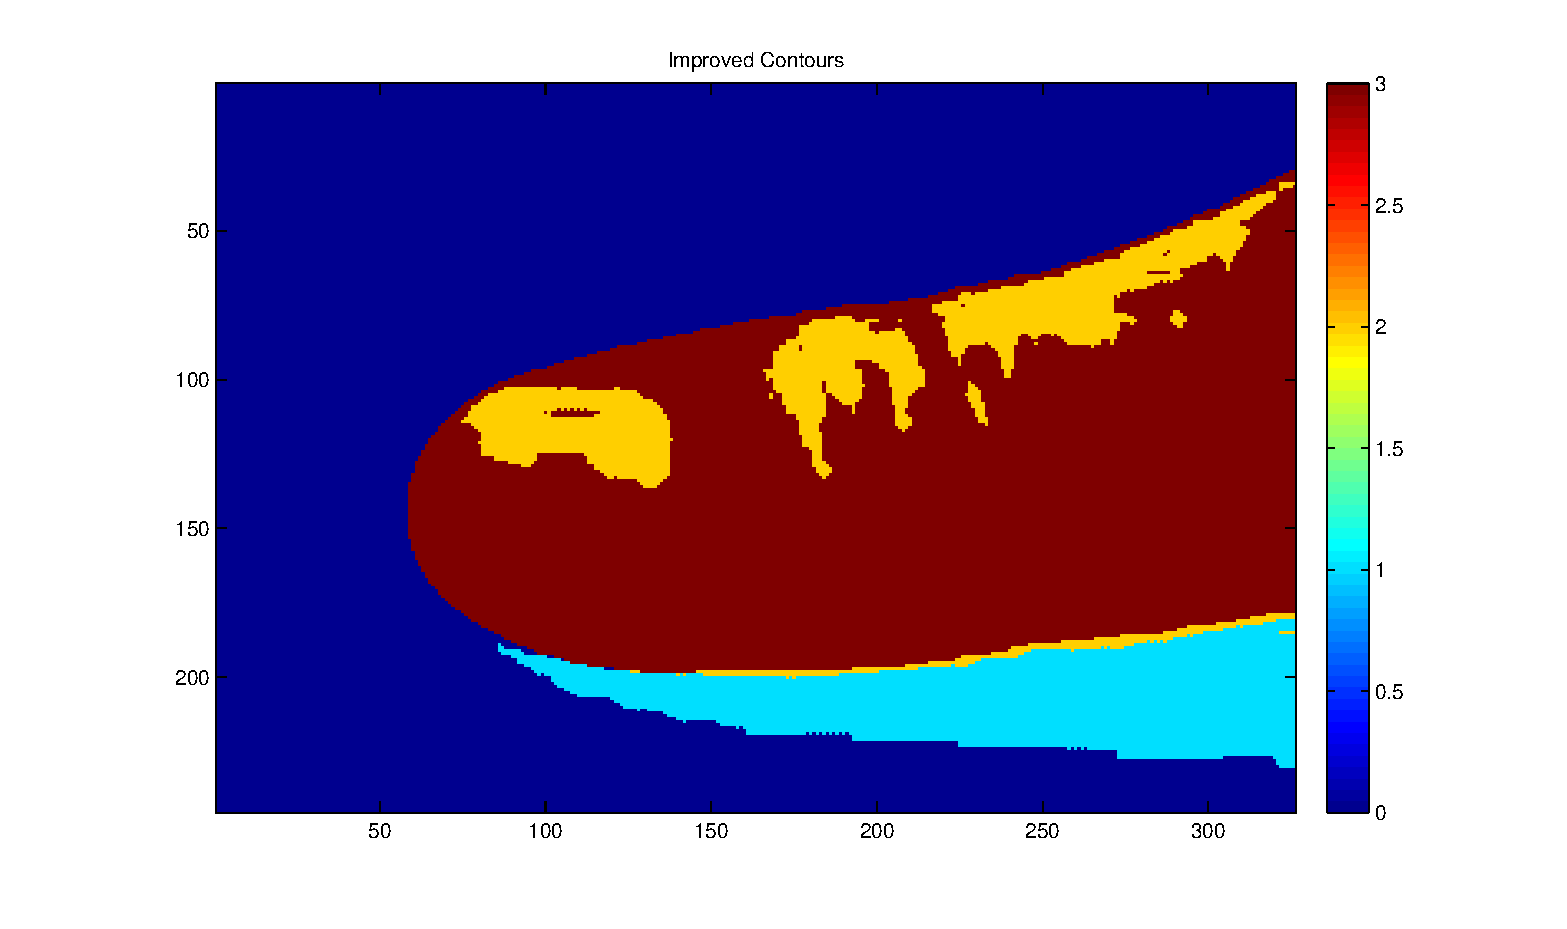
\includegraphics[width=0.70\textwidth]{Chapter3/Figs/2bitImage.eps}
    \caption{The improved contour method in action.}\label{fig:2BitImage}
\end{figure}

\section{Fingertip Descriptor}\label{sec:FingertipDescriptor}

Given that the SURF method fails to find any sort of reliable, small area features, we need a descriptor so we can accurately align points on the fingertip between successive images in the video stream. We need to do this because otherwise, any difference between the frames will be overwhelmed by physical movement of the digit rather than movement of the blood inside the digit. For this reason, we target the most stable portion of the finger: the nail. We have quite accurate tracking of the tip, so it's quite simple to place a point fairly centrally on a nail with no other information other than the position of the tip. We apply the Canny edge detector and find the edges which are radially located around that point. The radial edges are detected, which are used to align between frames. Essentially, they can be broken into four lines; two down the side being relatively straight. But it depends on the individual, and the digit. However, we know we're looking for something with a certain curvature, as well as the rough positions of the lines along the edges.

For each of those four lines, we have an orientation and a curvature, as well as the distance between the opposing lines. So, using that descriptor, we have the next frame, and in the new frame, we apply the Canny edge detector and detect four lines with similar characteristics. Given those edges, we can produce our best estimate, minimizing the difference between this frame and the previous one, in terms of their orientation and position. Based on this, we can work out a shift if there's been a change in position or orientation of the fingertip.

Because we're going from one frame to another in a video stream, the descriptor is sufficient to overlay the frames accurately to within a few pixel widths. Brute force feature matching can be used as a further refinement if necessary. For the purposes of detecting a finger press, however, this was not found to be necessary.

\section{Putting it All Together}\label{sec:PuttingItAllTogether}

So far, we have said little about how we actually intend to detect a digit being pressed on a surface. Although a significant amount of discussion has been presented to do with the optimization --- at least in terms of the data types and the underlying maths --- mostly to do with the color space transform. We have said even less about the size of the images captured or the framerate at which the processing is required. These are important considerations for designing practical code, especially for application in a mobile device.

\subsection{Detecting a Finger Press}\label{sec:DetectingAFingerPress}

In the previous section, we presented several algorithms which perform steps in the task. However, we now need to put them together and fill in the gaps which link each important step together. Assumptions and simplifications which we have allowed ourselves in this work which is intended only to be a proof of concept rather than a fully-fledged application. To this end, we have decided to simplify the requirements and --- although there is no compelling reason why we could not use, say, convex hull and defects to detect the fingers, or even a full hand --- we're only going to consider the case where one digit is presented to the routine in a controlled environment:

The first step in the algorithm is to select a human and a camera. With this done --- using the same camera as will be used by the application --- we gather statistics for a particular individual's skin, trying to vary the lighting conditions so as to give us as representative a data set as possible. From this, a color space is designed and the relevant transforms and such are instantiated for that particular individual.

The next step is to collect the finger features and instantiate the feature detectors using the Canny-edge-based descriptor for each of the individuals' digits.

Now we start the application: it turns on the camera and waits for movement. After the movement starts, it continues to wait until that movement slows, which is the first indicator that a surface is being touched. Here we assume that we are trying to detect static presses, so no pressing and dragging is considered. We look at a higher resolution frame, process that frame into the skin color space for the individual in question. 

Now we perform our shape detector, which looks for a finger-shaped object, finds the tip, creates rectangular bounds for the tip, and then takes an even higher resolution frame. (But only for the tip of the potential finger.) This image --- cropped to the tip of the digit --- is then sent to the feature detecton algorithm, which then uses the Canny edge feature method previously described and attempts to identify the digit by applying the known descriptors for the individual's nail.

These steps are relatively slow, but --- once applied --- the algorithm now only tries to fit one feature descriptor and simply tracks the assumed small movement of the tip during a press. Due to the slow nature of these steps, it's required that the camera buffers a few frames after the motion stops, otherwise the finger press may miss the processing window. It is at this stage that the algorithm to detect the finger press really starts.

Now that the fingertip has been located, the algorithm crops the fingertip before forming the color space transform, which saves a significant amount of processing time. We now define a larger cropping region, and a tight cropping region. The larger of the two cropping regions is used initially to ensure that the entire tip of the digit is captured in subsequent frames, as this cropping region will not vary during the finger press detection stage of the algorithm. Inside the cropping region, a second rectangular region is defined, which is centered using the feature detection, ensuring that the frames are aligned with the true outline of the digit and not the outer pixels. Any change in the tighter frame will be due to the mechanical action on the digit changing its visual appearance.

The tightly-cropped region from each frame is held in as high a resolution as possible, and the absolute distance between each successive frame is calculated in this region. It was discovered that the color channel corresponds to the major axis of the 2D Gaussian fit to the chromatic space. It has been found that a finger press changes the chromatic values in the end of the digit sufficiently for this to register clearly in this region. For the purposes of this project, this difference is calculated and output as an image. However, for the actual application, all that is required is a measure of the size of the change in the chromatic space.

\begin{figure}[h!]
  \centering
    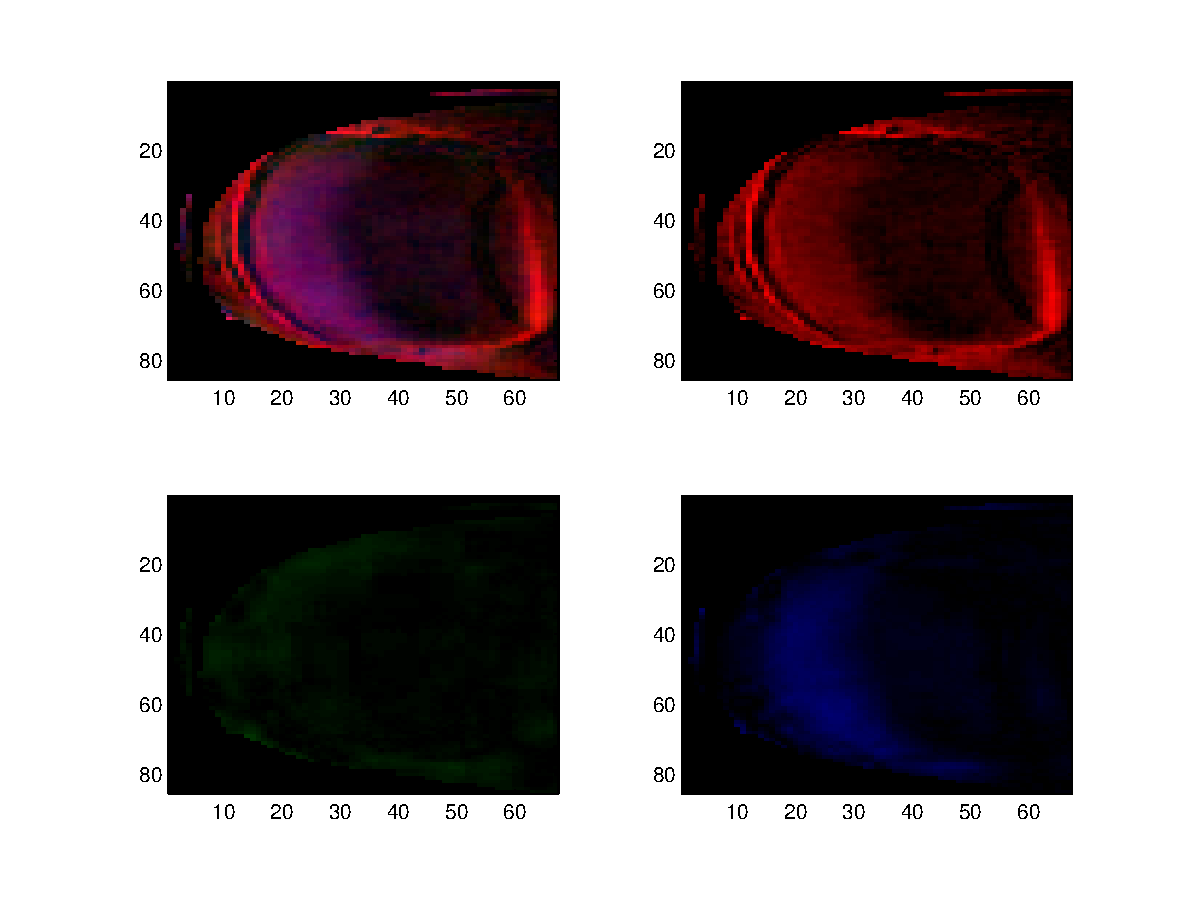
\includegraphics[width=0.90\textwidth]{Chapter3/Figs/jThumb_Final_Proof.eps}
    \caption{The difference in the skin color space between successive frames during a finger press. (Or in this case, a thumb.)}\label{fig:FinalProof}
\end{figure}

The second indicator for a finger press was found around the center of the pad of the digit. The distance to the convex hull --- which outlines the edge of the digit in the frame --- was noted to move away from the centered reference point. This is because the nail does not significantly deform under mechanical stress, however the soft tissue underneath does. This provides a second level in the metric for detecting a digit press.

The algorithm now decides based on thresholds which could be trained, but in the present implementation were set manually, one on the chromatic difference in the feature region (i.e. the nail), and the second on the contour from the shape detection. The output of each combined to produce a sound, the idea being the harder you press, the louder the noise.

The final step is to detect when the digit starts moving again. Failure of the feature detector to re-align the small frame makes the algorithm start tracking motion again. It looks at the low-resolution frames and sees if significant movement is occurring in the larger frame. It should be noted that the algorithm does not process outside of the larger cropped region during the finger press detection phase.
